\documentclass{article}
\usepackage{tikz}
\usetikzlibrary{external}
\usetikzlibrary{arrows}
%\tikzexternalize % activate!

\begin{document}
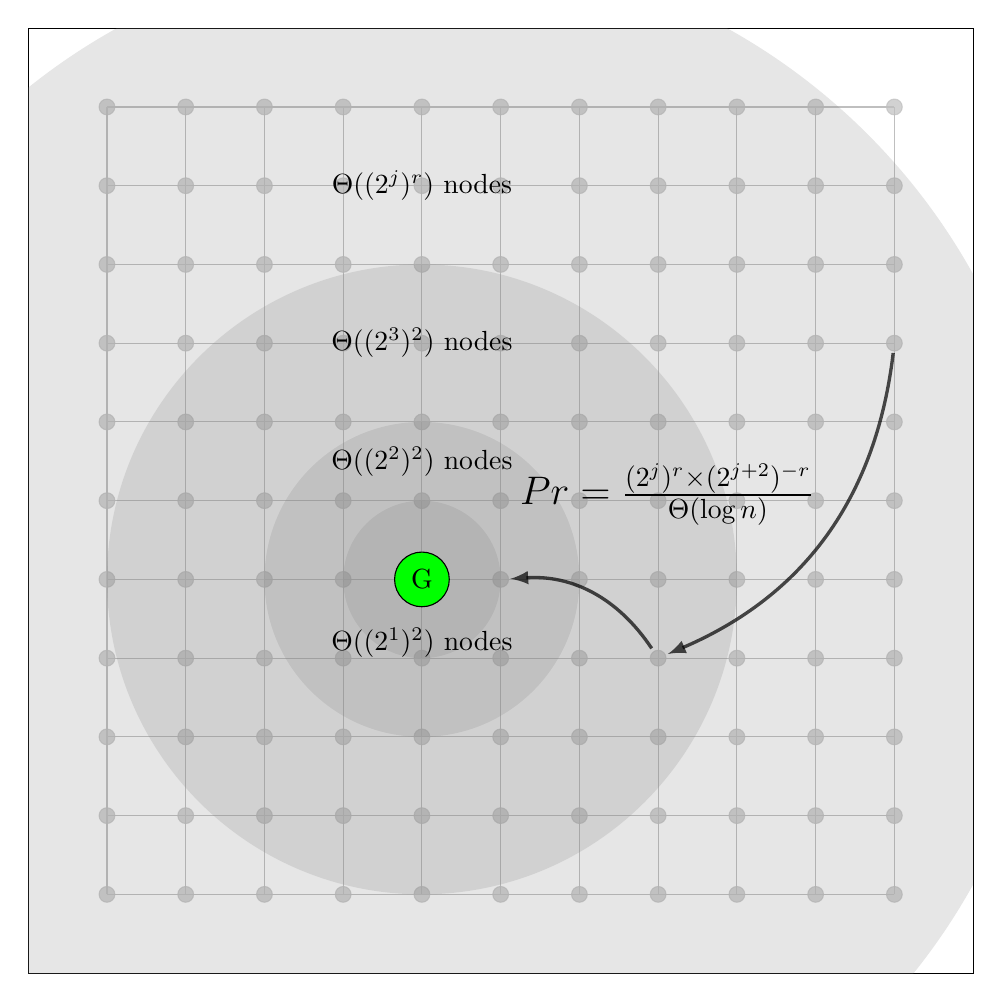
\begin{tikzpicture}[]
    % Grid
    \draw[clip] (-1,-1) rectangle (11,11);
    \draw[step=1,color=lightgray] (0,0) grid (10,10);
    \foreach \xpos in {0, 1, 2, 3, 4, 5, 6, 7, 8, 9, 10}
    {
      \foreach \ypos in {0, 1, 2, 3, 4, 5, 6, 7, 8, 9, 10}
      {
      \draw [color=lightgray,fill=lightgray,opacity=0.7] (\xpos,\ypos) circle (0.1);
      };
    };

    % Neighbourhoods
    \fill [fill=gray, opacity=0.2] (4,4) circle [radius=1];
    % Size 2
    \fill [fill=gray, opacity=0.2] (4,4) circle [radius=2];
    % Size 4
    \fill [fill=gray, opacity=0.2] (4,4) circle [radius=4];
    % Size 8
    \fill [fill=gray, opacity=0.2] (4,4) circle [radius=8];

    % Goal node
    \node (goal) [circle,draw,color=black,fill=green] at (4,4) {G};
    %\node (v1) (4,4)

    % Sizes
    \node at (4,3.2) {$\Theta((2^1)^2)$ nodes};
    \node at (4,5.5) {$\Theta((2^2)^2)$ nodes};
    \node at (4,7) {$\Theta((2^3)^2)$ nodes};
    \node at (4,9) {$\Theta((2^j)^r)$ nodes};

    % Hops
    \node (v0) at (10,7) {};
    \node (v1) at (7,3) {};
    \node (v2) at (5,4) {};
    \draw [overlay,-latex,very thick,opacity=0.7] (v0) 
        to [bend left] node[above left, opacity=1.0] 
        {\Large $Pr = \frac{(2^j)^r \times (2^{j+2})^{-r}}{\Theta(\log n)} $} (v1);
    \draw [overlay,-latex,very thick,opacity=0.7] (v1) to [bend right] (v2);



\end{tikzpicture}
\end{document}
